% tikzpic.tex
\documentclass[crop,tikz]{standalone}
\usetikzlibrary{calc,matrix,decorations.markings,decorations.pathreplacing}

\definecolor{colone}{RGB}{209,220,204}
\definecolor{coltwo}{RGB}{204,222,210}
\definecolor{colthree}{RGB}{207,233,232}

\definecolor{colfour}{RGB}{248,243,214}
\definecolor{colfive}{RGB}{245,238,197}
\definecolor{colsix}{RGB}{243,235,179}
\definecolor{colseven}{RGB}{241,231,163}

\tikzset{ 
  table/.style={
    matrix of nodes,
    row sep=-\pgflinewidth,
    column sep=-\pgflinewidth,
    nodes={rectangle,text width=2cm,align=center},
    text depth=1.25ex,
    text height=2.5ex,
    nodes in empty cells
  }
}

\renewcommand*{\familydefault}{\sfdefault}
\newcommand{\cbox}[1]{\parbox[t]{2cm}{\centering #1}}

%% http://www.texample.net/tikz/examples/arrow-table/

\begin{document}

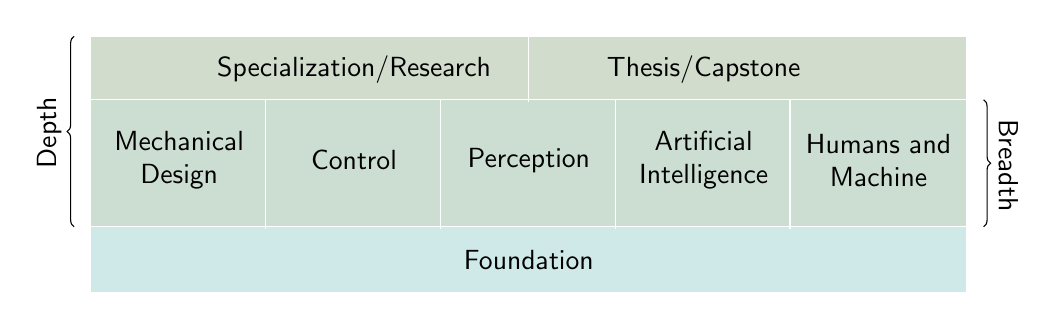
\begin{tikzpicture}
  \matrix (mat) [table] {
    |[fill=colone]|      & |[fill=colone]|  & |[fill=colone]|    & |[fill=colone]|  & |[fill=colone]|  \\
    |[fill=coltwo]|      & |[fill=coltwo]|  & |[fill=coltwo]|    & |[fill=coltwo]|  & |[fill=coltwo]|  \\
    |[fill=coltwo]|      & |[fill=coltwo]|  & |[fill=coltwo]|    & |[fill=coltwo]|  & |[fill=coltwo]|  \\
    |[fill=colthree]|       & |[fill=colthree]|   & |[fill=colthree]|     & |[fill=colthree]|   & |[fill=colthree]|   \\
  };

  % horizontal rules
  \foreach \row in {2,4}
  \draw[white] (mat-\row-1.north west) -- (mat-\row-5.north east);
  
  % \draw[white,ultra thick] (mat-1-1.north west) -- (mat-1-6.north east);
  % \draw[white,ultra thick] (mat-5-1.north west) -- (mat-5-6.north east);

  % vertical rules
  \foreach \col in {2,3,4,5}
    \draw[white] (mat-2-\col.north west) -- (mat-3-\col.south west);
  \draw[white] (mat-1-3.north) -- (mat-1-3.south);

  % The labels
  \node[fill=colone] at (mat-1-2) {Specialization/Research};
  \node[fill=colone] at (mat-1-4) {Thesis/Capstone};
  \node at ([yshift=-10pt]mat-2-1) {\cbox{Mechanical \\ Design}};
  \node at ([yshift=-10pt]mat-2-2) {\cbox{Control}};
  \node at ([yshift=-10pt]mat-2-3) {\cbox{Perception}};
  \node at ([yshift=-10pt]mat-2-4) {\cbox{Artificial \\ Intelligence}};
  \node at ([yshift=-10pt]mat-2-5) {\cbox{Humans and Machine}};
  \node[fill=colthree] at (mat-4-3) {Foundation};
  \node[rotate = 90] at ([xshift=-15pt]mat-2-1.west)
     {\textsf{Depth}};
  \node[rotate = -90] at ([xshift=15pt]mat-2-5.south east)
     {\textsf{Breadth}};
     
  % The braces
  \draw[decorate, decoration={brace, mirror, raise=6pt}]
    (mat-1-1.north west) -- (mat-4-1.north west);

  \draw[decorate, decoration={brace, mirror, raise=6pt}]
    (mat-4-5.north east) -- (mat-2-5.north east);
\end{tikzpicture}

\end{document}
